\begin{figure*}
\begin{center}
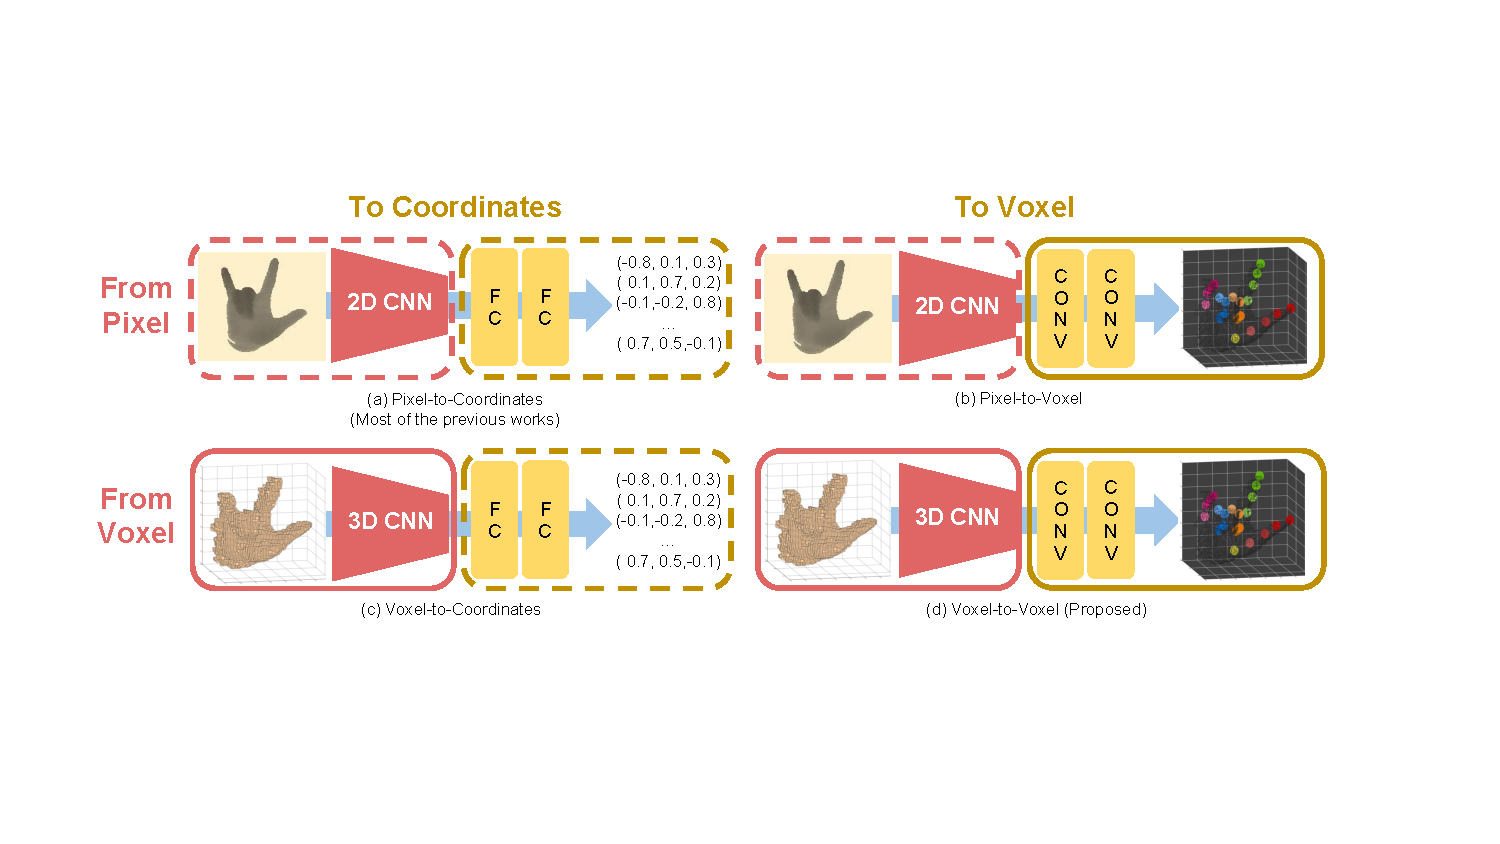
\includegraphics[width=1.0\linewidth]{comparison_io_type.pdf}
\end{center}
\vspace*{-5mm}
   \caption{Various combinations of inputs and outputs for 3D pose estimation from a single depth image. Most of the previous works take a 2D depth image as input and estimate the 3D coordinates of keypoints as in (a). In contrast, the proposed system takes a 3D voxelized grid and estimates the per-voxel likelihood of each keypoint as in (d). Note that (b) and (d) are solely composed of the convolutional layers that become the fully convolutional architecture.}
\label{fig:comparison_io_type}
\end{figure*}

\section{Related works}

{\bf Depth-based 3D hand pose estimation.} 
Hand pose estimation methods can be categorized into generative, discriminative, and hybrid methods. Generative methods assume a pre-defined hand model and fit it to the input depth image by minimizing hand-crafted cost functions ~\cite{sharp2015accurate, tang2015opening}. Particle swam optimization (PSO)~\cite{sharp2015accurate}, iterative closest point (ICP)~\cite{tagliasacchi2015robust}, and their combination~\cite{qian2014realtime} are the common algorithms used to obtain optimal hand pose results.

Discriminative methods directly localize hand joints from an input depth map. Random forest-based methods~\cite{keskin2012hand,tang2013real,tang2014latent,liang2014parsing,sun2015cascaded,tang2015opening,wan2016hand} provide fast and accurate performance. However, they utilize hand-crafted features and are overcome by recent CNN-based approaches ~\cite{tompson2014real,oberweger2015hands,ge2016robust,sinha2016deephand,bouchacourt2016disco,yang2016hand,deng2017hand3d,ge20173d,guo2017ren,guo2017towards,chen2017pose,madadi2017end,fourure2017multi,xu2017lie,Choi_2017_ICCV,Oberweger_2017_ICCV_Workshops} that can learn useful features by themselves. Tompson \etal~\cite{tompson2014real} firstly utilized CNN to localize hand keypoints by estimating 2D heatmaps for each hand joint. Ge \etal~\cite{ge2016robust} extended this method by exploiting multi-view CNN to estimate 2D heatmaps for each view. Ge \etal~\cite{ge20173d} transformed the 2D input depth map to the 3D form and estimated 3D coordinates directly via 3D CNN. Guo \etal~\cite{guo2017ren,guo2017towards} proposed a region ensemble network to accurately estimate the 3D coordinates of hand keypoints and Chen \etal~\cite{chen2017pose} improved this network by iteratively refining the estimated pose. Oberweger \etal~\cite{Oberweger_2017_ICCV_Workshops} improved their preceding work~\cite{oberweger2015hands} by utilizing recent network architecture, data augmentation, and better initial hand localization.

Hybrid methods are proposed to combine the generative and discriminative approach. Oberweger \etal~\cite{oberweger2015training} trained discriminative and generative CNNs by a feedback loop. Zhou \etal~\cite{zhou2016model} pre-defined a hand model and estimated the parameter of the model instead of regressing 3D coordinates directly. Ye \etal~\cite{ye2016spatial} used spatial attention mechanism and hierarchical PSO. Wan \etal~\cite{Wan_2017_CVPR} used two deep generative models with a shared latent space and trained discriminator to estimate the posterior of the latent pose.


{\bf Depth-based 3D human pose estimation.} 
Depth-based 3D human pose estimation methods also rely on generative and discriminative models. The generative models estimate the pose by finding the correspondences between the pre-defined body model and the input 3D point cloud. The ICP algorithm is commonly used for 3D body tracking~\cite{ganapathi2012real,grest2005nonlinear,knoop2006sensor,helten2013personalization}. Another method such as template fitting with Gaussian mixture models ~\cite{ye2014real} was also proposed. By contrast, the discriminative models do not require body templates and they directly estimate the positions of body joints. Conventional discriminative methods are mostly based on random forests. Shotton \etal~\cite{shotton2013real} classified each pixel into one of the body parts, while Girchick \etal~\cite{girshick2011efficient} and Jung \etal~\cite{jung2016sequential} directly regressed the coordinates of body joints. Jung \etal~\cite{yub2015random} used a random tree walk algorithm (RTW), which reduced the running time significantly. Recently, Haque \etal~\cite{haque2016towards} proposed the viewpoint-invariant pose estimation method using CNN and multiple rounds of a recurrent neural network. Their model learns viewpoint-invariant features, which makes the model robust to viewpoint variations.

\begin{figure*}
\begin{center}
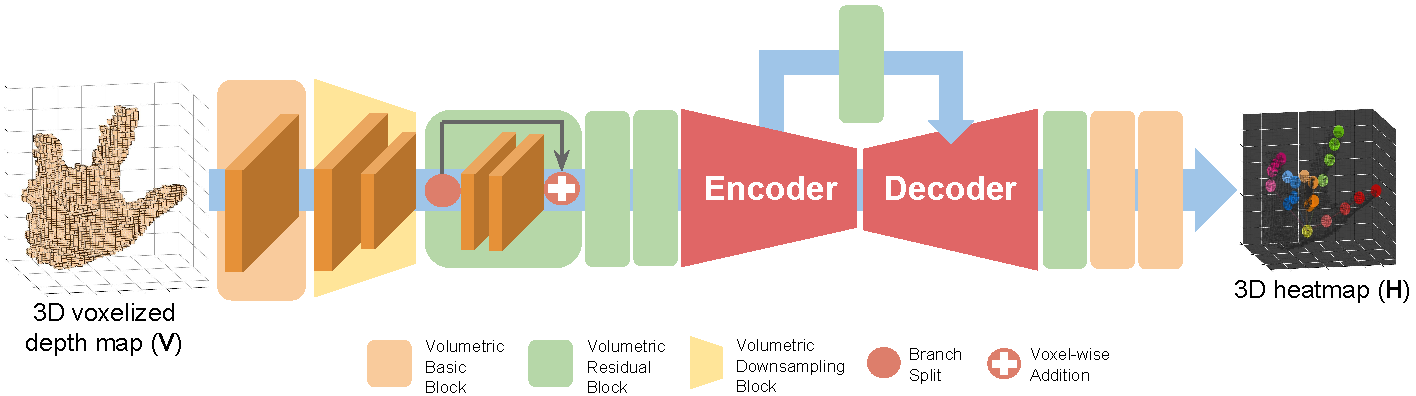
\includegraphics[width=1.0\linewidth]{model_architecture.pdf}
\end{center}
\vspace*{-5mm}
   \caption{Overall architecture of the V2V-PoseNet. V2V-PoseNet takes voxelized input and estimates the per-voxel likelihood for each keypoint through encoder and decoder. To simplify the figure, we plotted each feature map without Z-axis and combined the 3D heatmaps of all keypoints in a single volume. Each color in the 3D heatmap indicates keypoints in the same finger.}
\vspace*{-3mm}
\label{fig:model_architecture}
\end{figure*}

{\bf Volumetric representation using depth information.}
Wu \etal~\cite{wu20153d} introduced the volumetric representation of a depth image and surpassed the existing hand-crafted descriptor-based methods in 3D shape classification and retrieval. They represented each voxel as a binary random variable and used a convolutional deep belief network to learn the probability distribution for each voxel. Several recent works~\cite{maturana2015voxnet,song2016deep} also represented 3D input data as a volumetric form for 3D object classification and detection. Our work follows the strategy from ~\cite{maturana2015voxnet}, wherein several types of volumetric representation (i.e., occupancy grid models) were proposed to fully utilize the rich source of 3D information and efficiently deal with large amounts of point cloud data. Their proposed CNN architecture and occupancy grids outperform those of Wu \etal~\cite{wu20153d}.

{\bf Input and output representation in 3D pose estimation.}
Most of the existing methods for 3D pose estimation from a single depth map~\cite{oberweger2015hands,oberweger2015training,bouchacourt2016disco,Wan_2017_CVPR,guo2017ren,guo2017towards,Oberweger_2017_ICCV_Workshops,chen2017pose,madadi2017end,fourure2017multi,haque2016towards} are based on the model in Figure~\ref{fig:comparison_io_type}(a) that takes a 2D depth image and directly regresses 3D coordinates. Recently, Ge \etal~\cite{ge20173d} and Deng \etal~\cite{deng2017hand3d} converted a 2D depth image to a truncated signed distance function-based 3D volumetric form and directly regressed 3D coordinates as shown in Figure~\ref{fig:comparison_io_type}(c). In 3D human pose estimation from a RGB image, Pavlakos \etal~\cite{pavlakos2016coarse} estimated the per-voxel likelihood for each body keypoint via 2D CNN as in the Figure~\ref{fig:comparison_io_type}(b). To estimate the per-voxel likelihood from an RGB image, they treated the discretized depth value as a channel of the feature map, which resulted in different kernels for each depth value. In contrast to all the above approaches, our proposed system estimates the per-voxel likelihood of each keypoint via the 3D fully convolutional network from the voxelized input as in Figure~\ref{fig:comparison_io_type}(d). To the best of our knowledge, our network is the first model to generate voxelized output from voxelized input using 3D CNN for 3D pose estimation.








